%% =============================================================================
%% ОБЩИЕ ПРАВИЛА (для людей и для ИИ-агентов)
%% =============================================================================
%% 1. Это черновик ОДНОГО участника. Редактируй только этот файл.
%% 2. Не меняй чужие файлы в папке drafts/.
%% 3. Не трогай корневой main.tex, преамбулу, стили (.cls, .sty), .github/.
%% 4. Можно использовать существующие метки (\ref, \label, \cite), но не переименовывай их без согласования.
%% 5. Новые рисунки складывай в figures/ с уникальным именем: <имя>_<смысл>.png.
%% 6. Новые источники (BibTeX) пришли Давиду (david_final.tex) или в issues.
%% 7. Сохраняй статью в формате IEEEtran; не меняй шрифты/поля.
%% 8. После правки скинь файл координатору; сборка PDF делается в main.tex.
%% =============================================================================

%% УЧАСТНИК: Давид
%% РАЗДЕЛЫ: Examples of system operation... + Integration... + Use in control systems
%%          + Future development + Conclusion + Acknowledgment + Russian abstract
%% ЗАДАЧИ:
%%   - Переписать завершающие разделы своими словами.
%%   - Обновить рисунок OSTIS_in_control.png и все скриншоты OSTIS (pic_*.png).
%%   - Собрать и отформатировать новые BibTeX-записи от всех участников в bib/links.bib.
%%   - Проверить перекрёстные ссылки, dates, благодарности.
%%   - Abstract и keywords: переписать здесь и сообщить Глебу для согласования.
%% ЭТО САМАЯ МАЛЕНЬКАЯ ТЕКСТОВАЯ ЧАСТЬ; основная работа Давида — сборка и сверка.
%% =============================================================================

\section{Examples of system operation with natural language information display}

For information to be clear and understandable to the reader, it must be
presented consistently. The recipe authoring system interface allows the
structure of domains and ontologies to be expressed in natural language. This
process of converting an internal knowledge representation to an external
knowledge representation is performed by a graphical interface component.

\section{Integration of third-party solutions with a knowledge base}

A standard system built on the basis of OSTIS Technology can be easily
integrated with other systems in the workplace. To integrate
\textit{\textbf{ISA-88}}, \textit{\textbf{ISA-95}} and \textit{\textbf{ISA-5.1}}
standards system with other systems running on JSC ``Savushkin Product'', a
web-oriented approach is used --- the OSTIS server is accessed with the use of the
following queries:

\begin{lstlisting}[basicstyle=\small]
  http://industry.ostis.net?sys_id=unit
\end{lstlisting}

where ``sys\_id=unit'' defines a term (the name of an entity) whose value we want
to find out (in this example, in fact, the answer to the question ``What is a
\textit{unit}?''). This approach makes it relatively easy to add support for the
knowledge base in current control systems projects; it is enough to indicate the
names corresponding to the entities in the knowledge base within the control
system.

Thus, an interactive intelligent help system for control systems projects is
implemented, allowing employees to work with the control system and ask
questions directly during their tasks.

Another example is the integrated help subsystem within corporate Add-in
\textbf{EasyEPLANner} \cite{EasyEPLANner} for CAD EPLAN. It helps describe
technological objects (Tank, Boiler, etc.), operations, and so on according to
the \textit{\textbf{ISA-88}} standard. The UML-model of EasyEPLANner high-level
objects can be described in OSTIS. The \textbf{PID controller} is at the lower
level --- the control module. It can be replaced by the development
\textbf{Neuro-PID controller} with the connections to the units and other
high-level objects.

\section{Use in control systems}

It is very important to quickly and correctly react to different events during
process control, especially critical accidents. However, when we have a complex
distributed system, it is rather complicated and normally requires the help of a
human operator. This may lead to a variety of problems. Thus, using an
OSTIS-based system can help solve the issues described in Fig.~
ef{OSTIS_in_control}. For example, Project \#2 has a valve failure but does
not know what to do. It makes a request to the OSTIS server, which already knows
which projects also use this line (with this valve). The OSTIS server polls the
rest of the projects (projects \#1 and \#2). Each project has information about
which operations are currently active and provides an answer on what to do ---
pause the operation, do nothing, etc. After that, the OSTIS server sends back to
Project \#2 an answer with the resulting actions to be used. These actions are
performed automatically, without the need for a human operator.

\begin{figure}[ht]
  \centering
  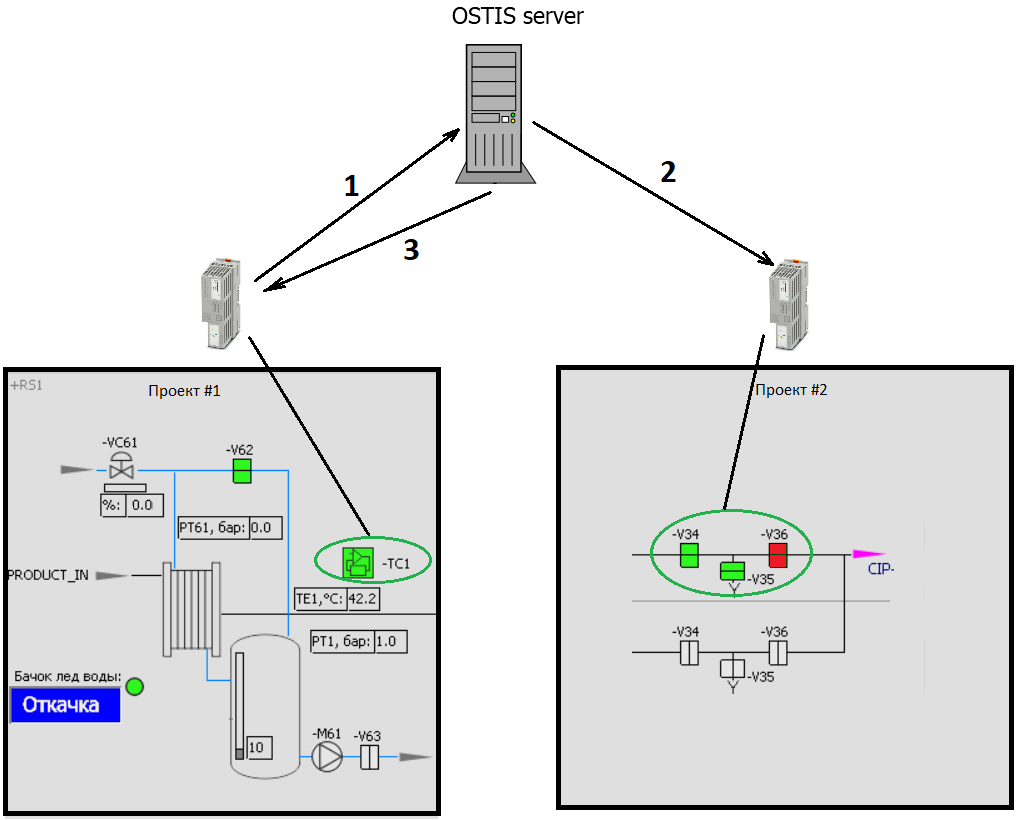
\includegraphics[width=0.45\textwidth]{figures/OSTIS_in_control.png}
  \caption{OSTIS in control systems}
  \label{OSTIS_in_control}
\end{figure}

\section{Future development}

Current project issues can be found on GitHub (\cite{EasyServer_4_0},
\cite{s88-ostis}, and \cite{isa-5.1-ostis}). The main problems to be solved are:
\begin{itemize}
  \item Improving system performance and especially accelerating system response
    time to user requests. This is connected with productivity and overall user
    satisfaction.
  \item Continuously updating and refactoring ontological models (further
    formalization of missing concepts, fixing typos, etc.).
  \item Enhancing PFC-visualization --- not only displaying but also editing
    diagrams. Adding rich navigation between PFC-diagrams and corresponding text
    representations.
  \item Further formulation of typical questions to the system from the user and
    their formalization at the level of the existing knowledge base.
  \item Adding detailed descriptions of real control projects based on the
    existing knowledge base.
\end{itemize}

The implementation of answers to complex questions is necessary to make the work
easier not only for process operators but also for maintenance personnel ---
instrumentation engineers, mechanics, electricians, etc. Therefore, it is
planned to implement the system's answer to the following type of question: in
what operations of which objects is this actuator used (for example, valve
\textbf{``T1V1''}). This question is very important when a device failure occurs,
and it is necessary to determine the criticality of this situation. For
analysis, it is necessary to compare the time of the accident and the history of
operations. For example, a failure of the mix-proof valve during the line
washing operation and the active product dosing along the other line should lead
to a stop of these operations and stop the preparation of the batch in the
corresponding unit. The operator must report this to the appropriate maintenance
specialist to fix it. After the fault has been eliminated, the operator
continues to perform operations. This is the correct order of events, which is
crucial to avoid mixing detergent and product. If the device malfunction
occurred within the line, which is now inactive, then this situation has a low
priority, does not lead to a halt in operations, and can be addressed later if
the service personnel have available time.

\section{Conclusion}

This paper considers a technique for automating the creation, development, and
use of standards based on OSTIS Technology. Using the example of the
\textit{\textbf{ISA-88}}, \textit{\textbf{ISA-95}}, and
\textit{\textbf{ISA-5.1}} standards implemented at the Savushkin Product
enterprise, it examines the knowledge base structure, the problem solver
features, and the support system user interface for these processes. The
developed system has been shown to integrate easily with other enterprise
systems, serving as a foundation for building an information service system for
employees within the context of Industry 4.0. The approach proposed in this work
not only automates the processes of creating, agreeing on, and developing
standards but also significantly increases the efficiency of applying standards
both manually and automatically.

\section*{Acknowledgment}

The author would like to thank the research teams of the Departments of
Intelligent Information Technologies at the Belarusian State University of
Informatics and Radioelectronics and the Brest State Technical University.

\bibliographystyle{bib/IEEEtran}
\balance
\bibliography{bib/links}

\bigskip
\begin{otherlanguage}{russian}
  \begin{center}
    \large\textbf{Нейро-символическое управление для пастеризационной установки}
    \medskip
    Иванюк Д.С.
  \end{center}

  \small
  В работе рассмотрен онтологический подход к пониманию, интеграции и развитию
  современных подходов к управлению (нейроуправление, большие языковые модели,
  современные международные стандарты) с использованием Технологии OSTIS.
  Уточнены формальные трактовки основных понятий, используемых в стандартах, что
  позволяет упростить описание реальных задач. Также описаны варианты интеграции
  базы знаний в используемые программные средства разработки и сценарии её
  использования непосредственно в системах управления.

\end{otherlanguage}

\medskip
\normalsize
\hfill Received May 15, 2026
\end{document}
